\chapter{Proposed Solution}

\begin{chapquote}{Jim Barksdale}
If we have data, let’s look at data. If all we have are opinions, let’s go with mine.
\end{chapquote}

\section{Introduction}

Perform a data-driven analysis required to develop a collection of tools
that are good enough to run in a lightning network node with daily activity. 
This section describes an open-source framework for the definition and 
the collection of lightning network metrics.

Therefore, in order to implement this framework an analysis of the state 
of the art was required (described in Section \ref{sec:problem_and_state_of_the_art})
to better understand what are the informations that are more difficult 
to get from a researcher's point of view.

From our preliminary study, we found that information on how a node performs 
on a daily basis are difficult to get, due to the following problems:
\begin{itemize}
    \item Requires a direct interaction with \emph{node operators};\footnote{node operators are people that own a 
        lightning node that point to help the network in routing payments.}
    \item Data collection of this kind can leak of private data, and node operators
        do not want be expose to this risk.
\end{itemize}

So, in order to work around these problems our proposal defines in a 
public manner what data will be collected, and how these are analyzed. This 
definition process is done through a lnmetrics Request for Comments (RFC) 
called \emph{lnmetrics RFC}. Then, after the data are defined, the collection 
of this data is done with a public server with public API with the possibility 
to self-hosting the server on hardware with at least a Raspberry PI 2 capability.

In addition, in order to incentivize node operators to provide and share the 
information with one of the public servers available we write the tool that 
collect the information on the lightning node with the possibility to run 
in an offline mode, and only if and when the node operators want the data 
are shared with one of the servers chosen (or more than one server).
One of the reasons that make the possibility to run in an offline mode a good
the incentive for node operators to be part of the research is that they 
are seeking a tool to analyze the node performance in order to increase the profit of
their node.

The Figure \ref{fig:lnmetrics_process} shows as the general process of propose 
a solution with our framework looks like.

\begin{figure}
    \begin{center}
      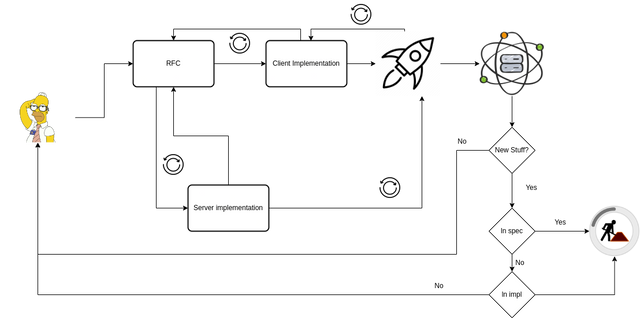
\includegraphics[scale=0.7]{imgs/lnmetrics-workflow-drawio.png}
    \end{center}
    \caption{Example of a process that uses lnmetrics.}
    \label{fig:lnmetrics_process}
\end{figure}

The suggested process to propose a new metrics described in the Figure \ref{fig:lnmetrics_process}
is composed by the following steps:

\begin{itemize}
    \item {\bf Data Definition}: Should be the first step of the process in order
        to clear define the scope of the data collection;
    \item {\bf Client Implementation}: After a first draft of the data mode is defined,
        the next step should be the implementation of the tools that is able to collect 
        the data. This step could required to can back to the previous step and change 
        somethings in the data model.
    \item {\bf Analysis Implementation}: Could be done in parallel to the Client implementation,
        and as in the client case the Analsys of the data collected can bring to rethink the data model
        and return to the stap 1.
    \item {\bf RFC proposal}: When the the data model and the code are in a stable phase,
        the metric can be proposed with an RFC and the discussion between the people interested
        can be done, this steps can require to introduce some change in one of more of the previous steps;
    \item {\bf Possible Proposal}: After the RFC is discussed the data analysis can bring to some 
        official proposal to the lightning network protocol or to one of the lightning networ implementation.
\end{itemize}

In the section \ref{sec:demo} the process of our case study is discussed.

\section{LNMetrics Request for Comments (RFC)}

The LNMetics Request for Comment (RFC) proposed is a more general idea of what 
it is already been done in the Lightning Network protocol definition. In fact,
this RFC is pointing to having the data description of what data are collected 
and how these data are used. It is not trying to define a 
standart of metrics for the lightning network, 
but more to incentivize discussion between people to achieve a better result.

\subsection{Data Definition}

Data definition is the most important part to propose a solution for a problem 
that required data analysis. Therefore, the data definition is a core 
part of the lnmetrics RFC process as the Figure \ref{fig:lnmetrics_process}
shows, and the process to propose a new \emph{metric} is composed from 
the following parts:

\begin{itemize}
    \item {\bf Metric Introduction}: An Introduction of the area that the metrics are targeting;
    \item {\bf Input Metric}: Data definition of the data that the researchers need. The data definition is done through a \emph{JSON schema}, and
    \item {\bf Output Metric}: Data definition of the data that the research point to return as a result. 
\end{itemize}

Ideally, the Metric proposal needs to be supported by a reference implementation to 
allow people to be part of the research by running the tool provided, and 
to support the RFC discussion.

However, at this time the problem on how to easily integrate new metrics inside the 
existing code is an open problem, and a possible solution is to allow the server 
to support a \emph{plugin protocol} that allow any person to extend the existing 
server with additional features.
In conclusion, when the new metric has been proposed inside the RFC a discussion between interested 
group of people need to be done in order to try to improve and verify the proposal, but if this is not possible
the proposal can be accepted directly by providing a reference implementation of the metrics proposed.

\section{Data Collection with LNMetrics Client}
\label{sec:lnmetrics_client}

A LNMetrics client is a generic concept of a tool that is able to collect one or more metrics 
defined inside the RFC, and allow a node operator or anyone that runs a lightning node
to collect data and share it with an analysis system described in Section \ref{sec:lnmetrics_server}.
In order to support our proposal a generic solution implemented in \emph{Go language} is provided 
and available on Github at \url{https://github.com/LNOpenMetrics/go-lnmetrics.reporter}, where we was able 
to provide a generic solution and allow the support of a generic metric concept 
by implementing the metric as interface defined as the Code \ref{code:lnmetric_client_inter} shows.

\begin{lstlisting}[language=go, basicstyle=\small,
                  caption={Metric interface provided in our client reference implementation.}, 
                  label={code:lnmetric_client_inter}]
// All the metrics need to respect this interface
type Metric interface {
    // return the unique name that the metrics has
    MetricName() *string
    // called when the metrics is initialized from 
    // the lightning node
    OnInit(lightning client.Client) error
    // called when the node is shutting down
    OnStop(msg *Msg, lightning client.Client) error
    // used to make the actual status of the metrics
    // persistent
    MakePersistent() error
    // called when the metrics is ready to be published
    UploadOnRepo(client *graphql.Client, 
        lightning client.Client) error
    // called when the metrics for the specific node 
    // need to be initialized on the server
    InitOnRepo(client *graphql.Client, 
        lightning client.Client) error
    // call that the lightning node use when it is 
    // time to update the metrics with new data
    Update(lightning client.Client) error
    // a more specific method to be able to call the 
    // update metrics with a specific message that allow 
    // to pass more information to the update method
    UpdateWithMsg(message *Msg, 
        lightning client.Client) error
    ToMap() (map[string]any, error)
    ToJSON() (string, error)
    // allow to perform data migration from an old 
    // data version to a new one
    Migrate(payload map[string]any) error
}
\end{lstlisting}

The LNMetrics client provided uses the core lightning plugin API
that allow us to easily integrate the client with the core lightning deamon 
and run the metrics client as part of the node itself. 
In addition, in order to allow an easy developmen of the plugin a 
Go API for core lightning is also provided, and available on 
Github at \url{https://github.com/vincenzopalazzo/cln4go}.

When the plugin is started a setup operation is performed, by creating a 
metrics database where the plugin make persistent the informations 
across node restarts, and also to support the offline mode feature. 
The database choosed is \emph{leveldb} that is a \emph{NO SQL} database 
that allow to store in an efficent way the data as key value and preserve
the disk space with a compression algorithm built-in the database itlsef.
In fact, our client implementation is havly based on the 
compression feature in order to preserve and allow anyone to 
run the tool. 

In the Figure \ref{fig:disk_space_servers} it is shows how much space is 
consumed by the database. 

\begin{figure}
    \begin{center}
    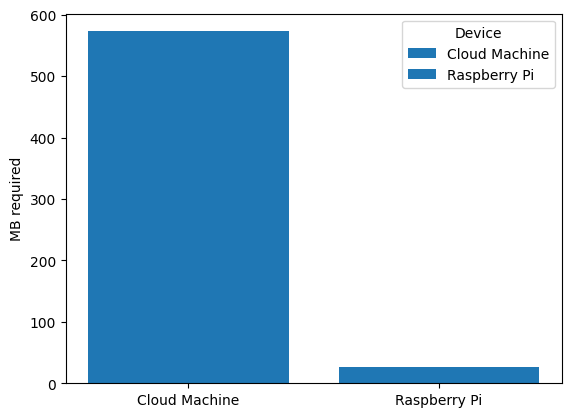
\includegraphics[scale=0.7]{imgs/disk_space_servers.png}
    \end{center}
    \caption{LNMetrics database size by istances.}
    \label{fig:lnmetrics_diskspace}
\end{figure}

\begin{itemize}
    \item {\bf Cloud machine}: Disk space consumed by the lnmetrics 
        sysytem on the cloud machine to store more that 1 year of metrics data;
    \item {\bf Raspberry PI 3}: Disk space consumed by the lnmetrics sysytem
        on a Raspberry PI to store 4 months of metrics data.
\end{itemize}

\section{LNMetrics Data Analsys}
\label{sec:lnmetrics_server}

After the data are collected by the LNMetrics client described in \ref{sec:lnmetrics_client}
our proposal is to aggregate the data in a server with public API where the data are 
public accessible to everyone. In this section there is a discussion of 
the server solution provided.

\subsection{Design Choise}

The choise to aggregare the data collected in a peer to peer system in a public 
server may sound a little bit odd, but the lnmetrics framework is designed in a 
way to keep every concept separate as the Figure \ref{fig:lnmetrics_architecture} 
shows. In fact the analysis sysytem is indipended from the report sysytem, and 
and the only information in common that this two sysytem need to have is the 
the data format, that it our design is done through the lnmetrics RFC.

\begin{figure}
    \begin{center}
    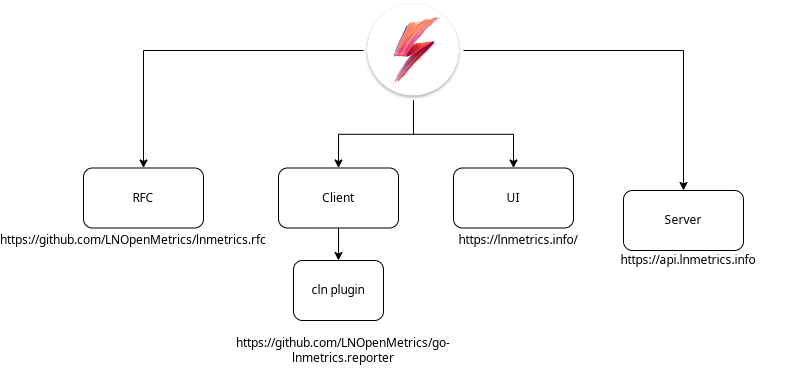
\includegraphics[scale=0.5]{imgs/lnmetrics-architecture.drawio.png}
    \end{center}
    \caption{LNMetrics architecture fesign diagram.}
    \label{fig:lnmetrics_architecture}
\end{figure}

Our choise to provide the lnmetrics server as method to analyze the data is to 
give one tool to organizzation and University to collect the data in a centralized
way to semplify the analysis step. However, our client implementation is able also
to compute the metric analysis also in the local envoirment and allow the own
of the node to inspec the result calculated without share the data with the centralized
server.

\subsection{API Description}

The server API use the \emph{GraphQL API} that allow an flexible way to fetch
a subpart of the data from the server. In particular, the GraphQL Protocol use
a concept of \emph{Query} where it is possible specify only the data that the 
caller want to know and avoid to receive all the JSON as response. This choice is to
improve the efficiency of the server, and speed up the performance. 

However, the downside of this approach is that with the GraphQL API the learning 
courve for a user is more hight that an normal Rest API, for this reason for our
case study a python library that implement a wrap of the server API is provided 
and an example of usage is given by a simple command line application 
available on Github at \url{https://github.com/LNOpenMetrics/py-lnmetrics.api}, 
where this command line tool is used to query the API periodically 
and store the data on the Github repository. 

Give the size of the database in the Figure \ref{fig:lnmetrics_diskspace}
storing a snapshot of the metrics as blob data in Github can be easily done, this allow 
to provide the data in another format and also to have a extra backup of the data 
in case of the server will brash or just reach the end of support from who is running it.

In conclusion, we provided an public API available at \url{https://api.lnmetrics.info} and 
a web site available at \url{https://lnmetrics.info} that privide access to the 
lnmetrics RFC, and some analsys on the case study described in the 
following sections.

\section{Local Reputation Metric}
\label{sec:demo}

In this section is described our case study that use the lnmetrics framework to 
define a local reputation of the node in order to provide a solution to a problem 
that we had while we was building our lightning node on the Bitcoin network.

So the local reputation described in this section is point to have some data 
in order to support a lightning network user during the initial phase that include 
discovery \emph{good lightning node} where it is possile to initialized a channel 
and also to discovery other node to increate the number of channel by analyze
the local view of our peers by having access to the server data.

\subsection{Data Definition}

The first step that we have done is to start to design our data model by analyze
the data that we was able to get from the core lightning node. Our first version
of the data model is available at the following link (TODO: put the link). 

Moreover the data are split in to main part divided as follow:

\begin{itemize}
    \item {\bf Lightning Node performance information}: The performance of the node that it is running
        the metrics, including
        \begin{itemize}
           \item Operative System information;
           \item The number of channels that the node has;
           \item The number of forwards payments that the node has performance the last 30 minutes
           \item The current lightning fee that the node has in order to forward a payment
        \end{itemize}
    \item {\bf Performance for each channel}:
    \begin{itemize}
        \item If the node is online at the moment of the check;
        \item The current lightning fee of the channel in order to forward a payment through it;
        \item The number of payment that are forwarded in the last 30 minutes through this specific 
            channel;
        \item The channel direction, so for each lightning channel there will be two item one of inbound connection, 
            and another one for outbound connection. In this way it is possible to try to estiamte what is the 
            usable direction of the channel.
    \end{itemize}
\end{itemize}

An more detailed descripion of the data is available on Github (TODO add link) where the
JSON schema is provided.

When the client push the data on the server the follwing metric output is calculated:

\begin{itemize}
    \item Lightning channel up time scoring divided by period is calculated;
    \item Lightning channel forwards payment scoring divided in \emph{success}, \emph{failure} and \emph{local failure}
        is calculated, where the local failure is how many forwards are failing caused to some lightning node problem,
        e.g the node that it is running the metrics has no channel with enough outbound capacity. 
    \item For each channel the previous information are calculated for this particular channel.
\end{itemize}

A more detailed description of the metric output is provided on Github as RFC with the JSON schema 
of the data just described. 

\subsection{Reference Implementation}

% FIXME: Describe how the plugin works under the hood

\subsection{Data Analsys}

% FIXME: Describe a little it how the data are analyzed
